% Appendix D

\chapter{Additional Tables and Figures} % Main appendix title

\label{AppendixD} % For referencing this appendix elsewhere, use \ref{AppendixA}

\section{Tables}

\begin{table}[H]
\caption{Polynomial Regression for European Call}{Polynomial regression result for the European call option}
\label{tab:fullEuroCall}
\centering
\begin{tabular}{llllllll}
\toprule
\textbf{Data set} &  \textbf{Measure} & \textbf{1. degree} & \textbf{2. degree} & \textbf{3. degree} & {4. degree} & \textbf{5. degree} & {6. degree}\\
\midrule
In-Sample     &	MSE  & 0.000636 & 0.000069 & 0.000013 & 0.000004 & 0.000002 & 0.000001 \\
		      & RMSE & 0.025212 & 0.008316 & 0.003624 & 0.002052 & 0.001414 & 0.000958 \\
		      & MAE  & 0.018326 & 0.006141 & 0.002561 & 0.001280 & 0.000867 & 0.000591 \\
		      & $R^2$& 0.936628 & 0.993105 & 0.998691 & 0.999580 & 0.999801 & 0.999909 \\
Long Maturity & MSE  & 0.002662 & 0.001196 & 0.001654 & 0.003956 & 0.012255 & 0.043361 \\
		      & RMSE & 0.051593 & 0.034577 & 0.040666 & 0.062894 & 0.110702 & 0.208233 \\
		      & MAE  & 0.041232 & 0.026287 & 0.028371 & 0.039932 & 0.064402 & 0.111190 \\
		      & $R^2$& 0.818143 & 0.918316 & 0.887014 & 0.729744 & 0.162742 & -1.962442 \\
Out-of-Money  & MSE  & 0.005772 & 0.000767 & 0.000839 & 0.000944 & 0.001812 & 0.004423 \\
		      & RMSE & 0.075973 & 0.027694 & 0.028960 & 0.030724 & 0.042568 & 0.066506 \\
		      & MAE  & 0.060936 & 0.022203 & 0.020288 & 0.020542 & 0.027125 & 0.041315\\
		      & $R^2$& -2.377251 & 0.551246 & 0.509280 & 0.447668 & -0.060261 & -1.588030\\
\bottomrule\\
\end{tabular}
\end{table}

\begin{table}[H]
\caption{Grid Search for American Bivariate Contingent Claim}{Hyperparameter tuning of dataset size and batch size for American put minimum two assets}
\label{tab:fullhyperAmerMin4}
\centering
\begin{tabular}{llll}
\toprule
\textbf{Data set Size} & \textbf{$\eta$} & \textbf{Batch Size} & \textbf{Train Loss} \\
\midrule
300K     & 0.0001 & 64   & 1.35215850605164E-06 \\ 
300K     & 0.001 & 64   & 2.1698210730392E-06 \\ 
300K     & 0.0001 & 8    & 2.73427281172189E-06 \\ 
300K     & 0.0001 & 256  & 2.94285678137385E-06 \\ 
300K     & 0.001 & 256  & 3.68489895663515E-06 \\ 
100K     & 0.0001 & 64   & 4.08099731430411E-06 \\ 
100K     & 0.001 & 64   & 4.81692904941156E-06 \\ 
100K     & 0.0001 & 256  & 5.18195474796812E-06 \\ 
300K     & 0.0001 & 1024  & 5.53397603653139E-06 \\ 
300K     & 0.001 & 8    & 5.79783136345213E-06 \\ 
300K     & 0.001 & 512  & 5.94204675508081E-06 \\ 
300K     & 0.0001 & 512  & 6.09576545684831E-06 \\ 
100K     & 0.0001 & 8    & 6.11733685218496E-06 \\ 
100K     & 0.001 & 256  & 7.29860903447843E-06 \\ 
100K     & 0.001 & 8    & 7.64047854318051E-06 \\ 
300K     & 0.001 & 1024  & 8.88059821591014E-06 \\ 
100K     & 0.0001 & 512  & 1.00699153335881E-05 \\ 
100K     & 0.001 & 512  & 1.02811236502021E-05 \\ 
300K     & 0.01  & 256  & 1.08374288174673E-05 \\ 
100K     & 0.001 & 1024  & 1.32220848172437E-05 \\ 
100K     & 0.0001 & 1024  & 1.34270530907088E-05 \\ 
300K     & 0.01  & 512  & 1.47791615745518E-05 \\ 
100K     & 0.01  & 256  & 1.87811801879434E-05 \\ 
100K     & 0.01  & 512  & 1.94587100850185E-05 \\ 
300K     & 0.01  & 64   & 2.06707663892303E-05 \\ 
100K     & 0.01  & 64   & 2.37144977290882E-05 \\ 
300K     & 0.01  & 1024  & 2.76203390967567E-05 \\ 
100K     & 0.01  & 1024  & 3.23796266457066E-05 \\ 
1K      & 0.0001 & 8    & 7.90390986367129E-05 \\ 
1K      & 0.001 & 8    & 0.000115903450933   \\ 
1K      & 0.001 & 64   & 0.0001487621048     \\ 
1K      & 0.0001 & 64   & 0.000176786270458   \\ 
1K      & 0.01  & 64   & 0.000234621096752   \\ 
1K      & 0.01  & 8    & 0.000340490310919   \\ 
1K      & 0.001 & 512  & 0.000384355953429   \\ 
1K      & 0.01  & 512  & 0.000385054125218   \\ 
1K      & 0.01  & 256  & 0.000567226845305   \\ 
1K      & 0.0001 & 256  & 0.000780252506956   \\ 
1K      & 0.001 & 256  & 0.000782921211794   \\ 
1K      & 0.0001 & 512  & 0.002630036789924   \\ 
1K      & 0.0001 & 1024  & 0.006931486539543   \\ 
1K      & 0.001 & 1024  & 0.012805146165192   \\ 
1K      & 0.01  & 1024  & 0.053760576993227   \\ 
100K     & 0.01  & 8    & 0.11506936699152    \\ 
300K                           & 0.01                        & 8                          & 35609.6484375                             \\
\bottomrule\\
\end{tabular}
\end{table}




\section{Figures}

\begin{figure}[H]
\centering
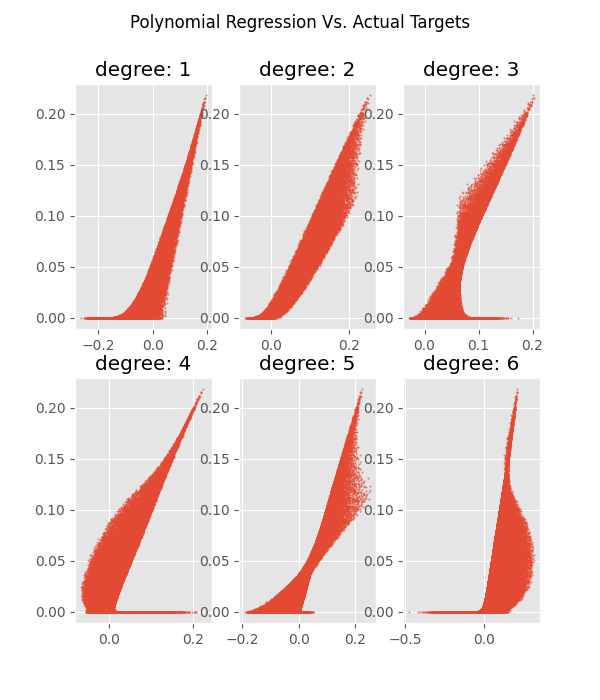
\includegraphics{Figures/polynomialOutMoneyEuroC.png}
\decoRule
\caption[Polynomial Regression Performance for Out-of-money Data Set European Call]{Polynomial regression performance for out of money data set on the European call}
\label{fig:MLPsEuroCOutOfMoney}
\end{figure}

\begin{figure}[th]
\centering
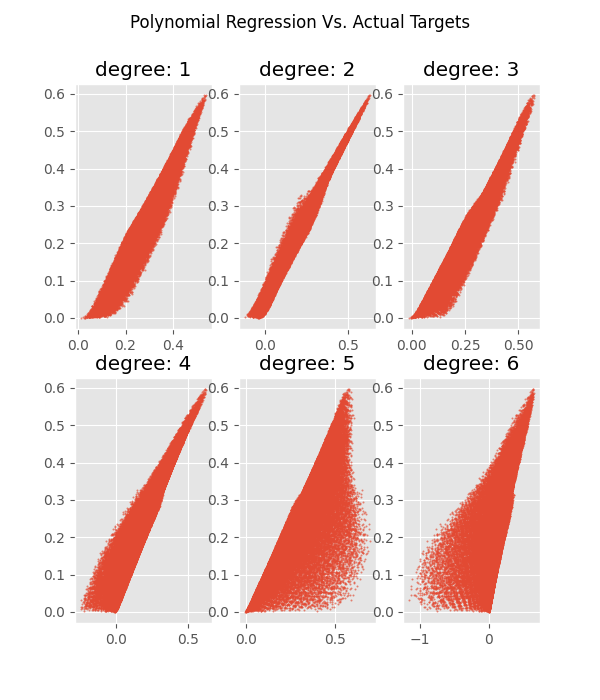
\includegraphics{Figures/polynomialLongTEuroC.png}
\decoRule
\caption[Polynomial Regression Performance for Long Maturity Data Set European Call]{Polynomial regression performance for long maturity data set on European call}
\label{fig:MLPsEuroCLongMaturity}
\end{figure}


\begin{figure}[th]
\centering
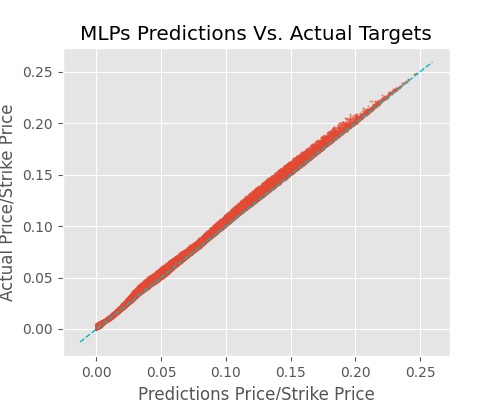
\includegraphics{Figures/outMoneyAmerP.png}
\decoRule
\caption[MLP Performance for In-the-Money Data Set American Put]{MLP performance for in-the-money data set on American put}
\label{fig:MLPsAmerPOutMoney}
\end{figure}

\begin{figure}[th]
\centering
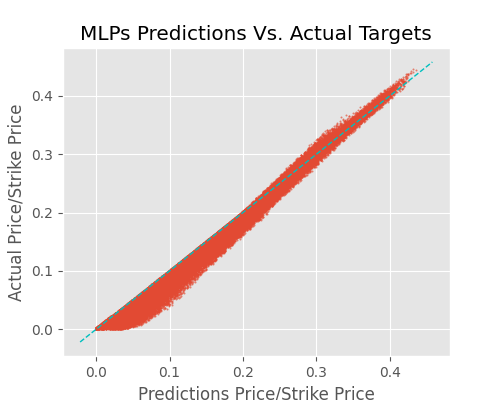
\includegraphics{Figures/longTAmerP.png}
\decoRule
\caption[MLP Performance for Long Maturity Data Set American Put]{MLP performance for long maturity data set on American put}
\label{fig:MLPsAmerPLongT}
\end{figure}

\begin{figure}[th]
\centering
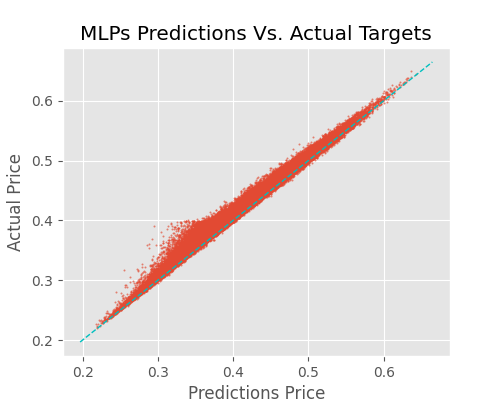
\includegraphics{Figures/inMoneyAmerMinP.png}
\decoRule
\caption[MLP Performance for In-the-Money Data Set Bivariate American Contingent Claim]{MLP performance on in-the-money data set on American put on minimum of two stocks}
\label{fig:MLPsAmerMin2}
\end{figure}

\begin{figure}[th]
\centering
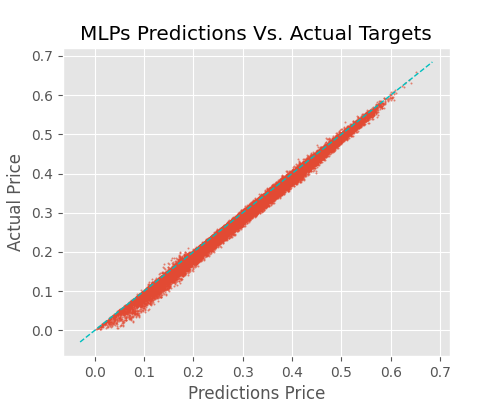
\includegraphics{Figures/longTAmerMinP.png}
\decoRule
\caption[MLP Performance for Long Maturity Data Set Bivariate American Contingent Claim]{MLP performance for long maturity data set on American put on minimum of two stocks}
\label{fig:MLPsAmerMin1}
\end{figure}






